%======================================================================================== 
%Preamble. Latex needs all this stuff to work, but it doesn't appear in your document.

\documentclass[onecolumn]{article}
\usepackage{natbib}
\usepackage{geometry}                
%\geometry{letterpaper} 
%\geometry{landscape}                
%\usepackage[parfill]{parskip}     % Activate to begin paragraphs with an empty line rather than an indent
\usepackage{graphicx}
\usepackage{amsmath}
\usepackage{amssymb}
\usepackage{float}
\floatstyle{plain}
\usepackage{listings}
\lstset{
    literate={~} {$\sim$}{1}
}
\usepackage{color}
\usepackage{epstopdf}
\usepackage[round]{natbib}
\usepackage{booktabs}
\usepackage{lipsum}
\newcommand{\eqname}[1]{\tag*{\bf #1}}% Tag equation with name
%\DeclareGraphicsRule{.tif}{png}{.png}{`convert #1 `dirname #1`/`basename #1 .tif`.png}
\usepackage{hyperref}
\hypersetup{
    colorlinks=true,
    linkcolor=blue,
    filecolor=magenta,      
    urlcolor=blue,
    citecolor={blue}
    }
%\usepackage{biblatex}
%========================================================================================  
% My title, name, and date
\title{My Title}
\author{My Name}
\date{The Date}                                         
%========================================================================================  


\begin{document}

\maketitle
\tableofcontents
\newpage

%==============This first section is just teaching you how to use LaTeX. It's not part of your paper.



\section{Using \LaTeX}

\subsection{Installing \LaTex}

Installation is easy. For MacOS, just download from \href{http://www.tug.org/mactex/}{here}. For Windows, look \href{http://www.howtotex.com/howto/installing-latex-on-windows/}{here}.

\subsection{Useful \LaTeX commands}

\begin{enumerate}
\item To use this section, look at the .tex file itself, rather than just this PDF. It contains the scripts that do the work.
\item Sections are made using the command used to make this section. You can also have subsections and subsubsections. \LaTeX will automatically number them for you. 
\item Lots of commands in \LaTeX do something to text between curly brackets. If your document fails to compile, it's almost always because you've forgotten to close with a curly bracket. Compile frequently so that you can easily track down the error.
\item Paragraphs. Leave a double space between lines (double carriage return). Or insert two backslashes at the end of the line.
\item Enumerate: The enumerate commands make a list such as this one. For a unnumbered list, use ``itemize'' rather than ``enumerate''
\item Quotes: To open quotes, use the ``\textbf{`}" key below the tilde twice. To close them, use the regular double quotes key once. I know, it's mad, but there it is.
\item Italics: \emph{italics}. Always italicize worm gene names, e.g., \emph{mab-3}.
\item Math: is the thing that \LaTeX is really good at. I'll give you an example of an equation below, but you probably won't need it.
\item Figures: Their size, shape and position can be elaborately specified, but keep it simple.
\item Citations: work like this: \cite{Lee2008} or \citep{Levin2012}. Now, to make them work you need to have a Bibtex file containing your citations. I have given you one to start with called ``Wormreferences". Bibtex formatted references can be downloaded easily from marked lists in Web of Knowledge. Just copy and paste your references into the ``References file''. The actual format of the references is given in the bibstyle commands at the end of the document. Don't mess with that. It's not exactly Harvard---but getting exactly Harvard is a whole other story.
\item Citations \emph{continued}. To format the citations in your document, you have to compile it once, run the Bibtex command under ``Typeset'', and compile it again. If it doesn't work, do it a few times and they'll pop up nicely formatted.
\item Citations \emph{continued}. To get the proper caps and italics in your references you need specify them in the ``references file''. Putting something in curly brackets will enforce caps; italicize as you would in a document (see examples). 
\item Hyperlinks. Can be done like this: \href{http://www.wormbase.org/}{Wormbase}.
\item Dashes. The best kind of dash to use needs three keyboard hyphens in a row---like this.
\item Ancillary files: Your figure and reference file needs to be in the same folder as your main text file---or you have to specify it's in a different one.
\item Figures: They should be PDFs or jpgs. TIFFs won't work.
\item Have \textbf{patience}! If you can't figure something out, just Google it, and you're sure to find an answer.
\item Finally, trust me---this will be worth it. Just---please---don't try to learn \LaTeX  the night before the essay is due.
\end{enumerate}

\subsection{Figures, Tables \& Equations}

You can put figures directly into the text. If you want to mess with their formatting, look \href{http://en.wikibooks.org/wiki/LaTeX/Floats,_Figures_and_Captions}{here}.

\floatstyle{plain}
\restylefloat{figure}
\begin{figure}[h]
\centering
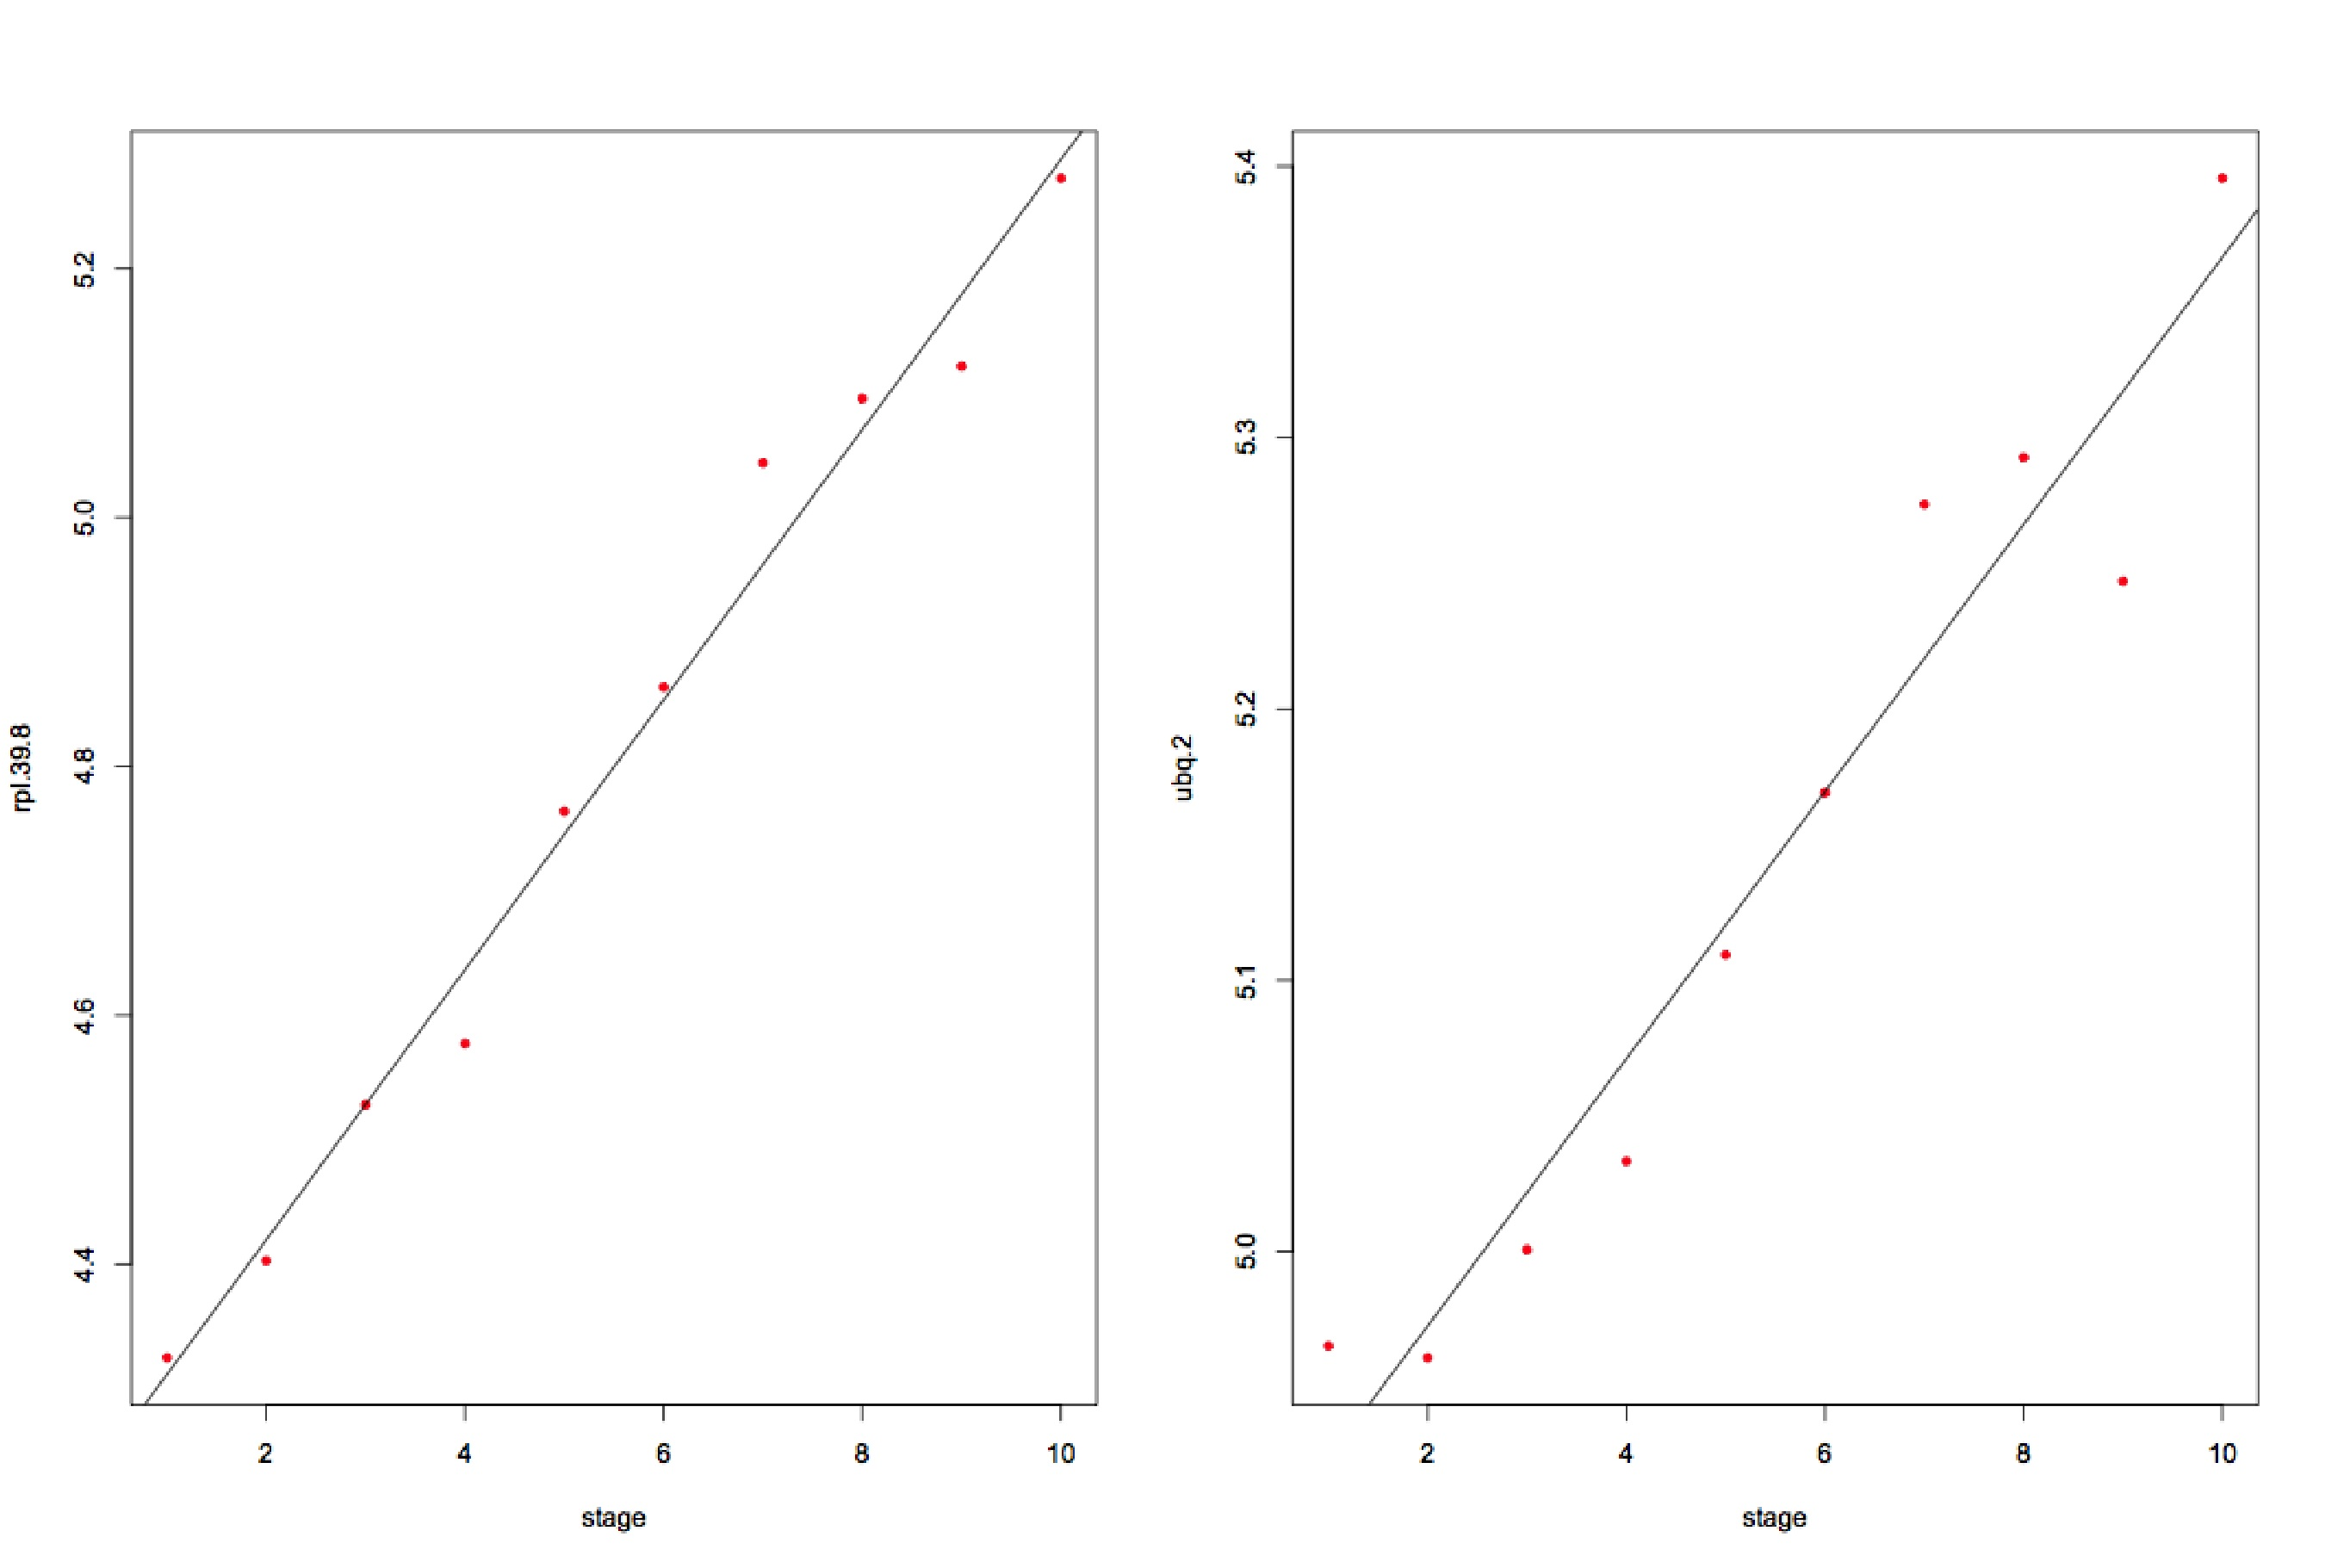
\includegraphics[width=7cm]{rpl}
\caption{\emph{rpl} gene expression in \emph{C. elegans} development}
\label{fig:rpl}
\end{figure}

I have to say that Figure \ref{fig:rpl} is a bit of a rubbish figure. You should generate better ones in R by playing with the plot settings---or use the ggplot2 library. It's very nice, but has quite a steep learning curve. \LaTeX is pretty good about placing figures, but of course if it doesn't have the space on a page, it will put it somewhere that you may not want it. You'll just have to experiment. 


Here is how to make a table such as Table \ref{table:things table}:
\begin{table}[ht]
\begin{center}
\begin{tabular}{lrrrrr}%{| p{1cm} | p{1cm} | p{1cm} |p{1cm} |p{1cm} |p{1cm}|}
\hline
Things&$r$&$r'$&$n$&$n'$&$w_i$\\
\hline
A&10&1&1&10&10 \\
B&10&6&1&5&5\\
C&10&3&1&8&8\\
D&10&2&1&9&9\\
E&10&5&1&6&6\\
\bottomrule
\\
\end{tabular}
\caption{The Table's title}
\label{table:things table}
\end{center}
\end{table}

And, finally, here is how to make an equation such as Equation \ref{eqn: nonlin}. These can be as complicated as you please. 

\begin{equation}
\Delta SD(z)= \Var(z_i-\bar z)^2\beta\left(\frac{w_i}{\bar w}, (z_i-\bar z)^2\right)
\label{eqn: nonlin}
\end{equation}

% This is just a way of putting in rubbish text and should be removed when you write.
\newpage
\section{Introduction}


\subsection{A subsection}
Your actual paper starts here. Just type away, using the commands above to format the thing. Don't worry if it crashes---\LaTeX never loses anything.
\subsubsection{A subsubsection}

\section{Methods}

Write about the methods you used.  You don't have to give R code, just tell me what packages you used, and if you did anything special tell me what. Nor do you have to use these subsections---they're just examples. 

\subsection{Identifying my genes of interest}
\subsection{Heatmap and Hierarchal Cluster Analysis}
\subsubsection{Heatmap}
\subsubsection{Hierarchal Cluster Analysis}
\subsection{Network Construction}

\section{Results}
\subsection{\emph{rpl} gene expression increases during development}

Each of your results subsections should be a simple declarative sentence, like the one that starts this subsection.

\section{Discussion}
\section{Conclusions}

\newpage
%Bibliography style
\newpage
\bibliography{Wormreferences}
\bibliographystyle{authordate1}

\end{document}  
















































